\scalebox{0.75}{
 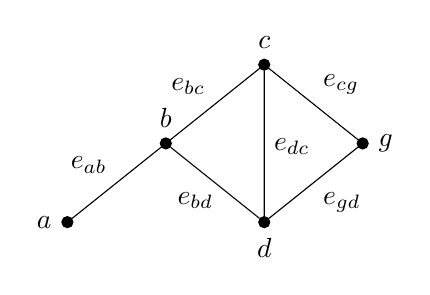
\begin{tikzpicture}[scale=1.0]
    \tikzstyle{N}=[draw,circle,fill=black,minimum size=4pt,inner sep=0pt]
    \draw (0,0) node (a) [N,label=left:$a$] {}
          to node[midway,auto] {$e_{ab}$} ++(1.25cm,1.0cm) node (b) [N,label=above:$b$,\VCShow] {}
          to node[midway,auto] {$e_{bc}$} ++(1.25cm,1.0cm) node (c) [N,label=above:$c$] {}
          to node[midway,auto] {$e_{cg}$} ++(1.25cm,-1.0cm) node (g) [N,label=right:$g$,\VCShow] {}
          to node[midway,auto] {$e_{gd}$} ++(-1.25cm,-1.0cm) node (d) [N,label=below:$d$,\VCShoww] {}
          to node[midway,right] {$e_{dc}$} (c)
          ;
   \draw (b) to node[midway,below] {$e_{bd}\hspace*{0.5cm}$} (d);
 \end{tikzpicture}
}
